\documentclass[11pt,a4paper]{article}

% Packages
\usepackage[utf8]{inputenc}
\usepackage[T1]{fontenc}
\usepackage{lmodern}
\usepackage[margin=2.5cm]{geometry}
\usepackage{graphicx}
\usepackage{xcolor}
\usepackage{listings}
\usepackage{hyperref}
\usepackage{booktabs}
\usepackage{longtable}
\usepackage{tikz}
\usepackage{fancyhdr}
\usepackage{tcolorbox}
\usepackage{enumitem}

% TikZ libraries
\usetikzlibrary{shapes.geometric, arrows.meta, positioning, fit, backgrounds}

% Colors
\definecolor{claudeblue}{RGB}{114, 162, 247}
\definecolor{codexgreen}{RGB}{16, 163, 127}
\definecolor{miyabipurple}{RGB}{147, 112, 219}
\definecolor{codebg}{RGB}{245, 245, 250}
\definecolor{linkcolor}{RGB}{0, 102, 204}

% Hyperref setup
\hypersetup{
    colorlinks=true,
    linkcolor=linkcolor,
    urlcolor=linkcolor,
    citecolor=linkcolor
}

% Listings setup
\lstset{
    basicstyle=\ttfamily\small,
    backgroundcolor=\color{codebg},
    frame=single,
    framerule=0.5pt,
    rulecolor=\color{gray!50},
    breaklines=true,
    breakatwhitespace=true,
    showstringspaces=false,
    tabsize=2,
    xleftmargin=1em,
    xrightmargin=1em,
    aboveskip=1em,
    belowskip=1em
}

% Header/Footer
\pagestyle{fancy}
\fancyhf{}
\fancyhead[L]{\textcolor{miyabipurple}{\textbf{Miyabi}} CCG/CG Coordination}
\fancyhead[R]{\thepage}
\fancyfoot[C]{\footnotesize\textcolor{gray}{Miyabi Multi-Agent Orchestration Architecture}}

% Custom boxes
\newtcolorbox{infobox}[1][]{
    colback=claudeblue!10,
    colframe=claudeblue,
    fonttitle=\bfseries,
    title=#1
}

\newtcolorbox{warningbox}[1][]{
    colback=orange!10,
    colframe=orange!80!black,
    fonttitle=\bfseries,
    title=#1
}

\newtcolorbox{codexbox}[1][]{
    colback=codexgreen!10,
    colframe=codexgreen,
    fonttitle=\bfseries,
    title=#1
}

% Title
\title{
    \vspace{-2cm}
    \textcolor{miyabipurple}{\Huge\textbf{Miyabi}}\\[0.5em]
    \Large Claude Code \& Codex\\
    \large Multi-Agent Coordination Architecture\\[1em]
    \normalsize CCG (Claude Code Guide) + CG (Codex Guide) Subagent System
}
\author{Miyabi Development Team}
\date{November 2025}

\begin{document}

\maketitle
\thispagestyle{empty}

\begin{abstract}
This document provides a comprehensive technical specification for coordinating Claude Code (CCG) and OpenAI Codex (CG) agents within the Miyabi autonomous development platform. We detail the subagent architectures of both systems, define coordination patterns, and establish best practices for multi-agent orchestration. The goal is to enable hybrid AI development workflows that leverage the strengths of both Claude and OpenAI models.
\end{abstract}

\tableofcontents
\newpage

%==============================================================================
\section{Introduction}
%==============================================================================

\subsection{Miyabi Platform Overview}

Miyabi is a complete autonomous AI development operations platform implementing:

\begin{itemize}[leftmargin=2em]
    \item \textbf{GitHub-as-OS}: Issues = Tasks, PRs = Deliverables, Actions = CI/CD
    \item \textbf{21 AI Agents}: 7 coding agents + 14 business agents
    \item \textbf{59 Rust Crates}: Modular architecture with 50\%+ faster compilation
    \item \textbf{28+ MCP Servers}: Extensible tool ecosystem
    \item \textbf{A2A Protocol}: Agent-to-Agent communication standard
\end{itemize}

\subsection{CCG and CG Definition}

\begin{table}[h]
\centering
\begin{tabular}{lll}
\toprule
\textbf{Abbreviation} & \textbf{Full Name} & \textbf{Description} \\
\midrule
CCG & Claude Code Guide & Claude Code subagent system \\
CG & Codex Guide & OpenAI Codex subagent system \\
\bottomrule
\end{tabular}
\caption{Agent System Abbreviations}
\end{table}

\subsection{Document Objectives}

\begin{enumerate}
    \item Define CCG and CG subagent capabilities and limitations
    \item Establish coordination patterns for hybrid workflows
    \item Provide implementation guidelines for Miyabi integration
    \item Document best practices for multi-agent orchestration
\end{enumerate}

%==============================================================================
\section{Claude Code (CCG) Architecture}
%==============================================================================

\subsection{Core Mechanism}

Claude Code's Task tool operates as an ephemeral worker spawning system:

\begin{itemize}
    \item Each Task receives an \textbf{isolated 200k context window}
    \item Subagents maintain \textbf{independent state} from parent
    \item Maximum \textbf{10 concurrent tasks} in parallel
    \item \textbf{No nested subagents}: Subagents cannot spawn other subagents
\end{itemize}

\begin{figure}[h]
\centering
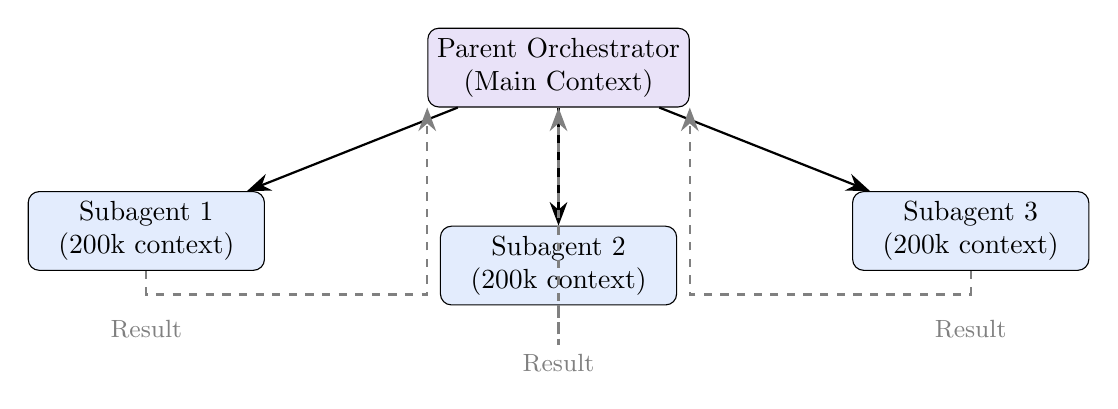
\begin{tikzpicture}[
    node distance=1.5cm,
    box/.style={rectangle, draw, rounded corners, minimum width=3cm, minimum height=1cm, align=center},
    arrow/.style={-{Stealth[length=3mm]}, thick}
]
    % Parent
    \node[box, fill=miyabipurple!20] (parent) {Parent Orchestrator\\(Main Context)};

    % Subagents
    \node[box, fill=claudeblue!20, below left=of parent, xshift=-1cm] (sub1) {Subagent 1\\(200k context)};
    \node[box, fill=claudeblue!20, below=of parent] (sub2) {Subagent 2\\(200k context)};
    \node[box, fill=claudeblue!20, below right=of parent, xshift=1cm] (sub3) {Subagent 3\\(200k context)};

    % Arrows
    \draw[arrow] (parent) -- (sub1);
    \draw[arrow] (parent) -- (sub2);
    \draw[arrow] (parent) -- (sub3);

    % Results
    \node[below=0.5cm of sub1, text=gray, font=\small] {Result};
    \node[below=0.5cm of sub2, text=gray, font=\small] {Result};
    \node[below=0.5cm of sub3, text=gray, font=\small] {Result};

    % Arrows back
    \draw[arrow, dashed, gray] (sub1.south) -- ++(0,-0.3) -| (parent.south west);
    \draw[arrow, dashed, gray] (sub2.south) -- ++(0,-0.5) -- (parent.south);
    \draw[arrow, dashed, gray] (sub3.south) -- ++(0,-0.3) -| (parent.south east);
\end{tikzpicture}
\caption{CCG Subagent Execution Model}
\end{figure}

\subsection{Built-in Subagent Types}

\begin{table}[h]
\centering
\begin{tabular}{llll}
\toprule
\textbf{Type} & \textbf{Model} & \textbf{Tools} & \textbf{Use Case} \\
\midrule
General-Purpose & Sonnet & All & Full-stack implementation \\
Plan & Sonnet & Read-only & Architecture analysis \\
Explore & Haiku & Read-only & Fast codebase discovery \\
claude-code-guide & --- & Docs & Documentation lookup \\
\bottomrule
\end{tabular}
\caption{CCG Built-in Subagent Types}
\end{table}

\subsection{Custom Subagent Configuration}

Custom subagents are defined via YAML frontmatter in Markdown files:

\begin{lstlisting}[language=yaml, caption=Custom CCG Subagent Definition]
---
name: security-reviewer
description: "Security audit specialist"
model: sonnet
tools:
  - Read
  - Glob
  - Grep
  - Bash
permissionMode: default
---

You are a security expert analyzing code for vulnerabilities...
\end{lstlisting}

\textbf{Storage Locations:}
\begin{itemize}
    \item Project-level: \texttt{.claude/agents/} (version-controlled)
    \item User-level: \texttt{\textasciitilde/.claude/agents/} (global)
\end{itemize}

\subsection{Claude Agent SDK Architecture}

\begin{infobox}[SDK Components]
\begin{itemize}
    \item \texttt{ClaudeSDKClient}: Stateful multi-turn sessions
    \item \texttt{query()}: Stateless one-off queries
    \item \texttt{ClaudeAgentOptions}: Configuration object
    \item Hooks: PreToolUse, PostToolUse, SessionStart, etc.
\end{itemize}
\end{infobox}

\subsubsection{Python SDK Usage}

\begin{lstlisting}[language=python, caption=Claude Agent SDK Example]
from claude_agent_sdk import ClaudeSDKClient, ClaudeAgentOptions

options = ClaudeAgentOptions(
    allowed_tools=["Read", "Write", "Bash"],
    model="sonnet",
    permission_mode="acceptEdits",
    max_turns=20
)

async with ClaudeSDKClient() as client:
    await client.connect(initial_prompt)
    async for message in client.query(task):
        process_message(message)
\end{lstlisting}

\subsection{Communication Patterns}

\textbf{Key Principles:}
\begin{enumerate}
    \item Subagents receive \textbf{only task-relevant context}
    \item Results return to parent \textbf{without context pollution}
    \item \textbf{No peer-to-peer communication} between subagents
    \item Orchestrator maintains \textbf{separation of concerns}
\end{enumerate}

%==============================================================================
\section{OpenAI Codex (CG) Architecture}
%==============================================================================

\subsection{Core Mechanism}

Codex CLI integrates via Model Context Protocol (MCP) server architecture:

\begin{itemize}
    \item Exposes \texttt{codex()} and \texttt{codex-reply()} tools
    \item Persistent session across agent turns
    \item Configurable sandbox and approval policies
    \item Native Agents SDK integration
\end{itemize}

\begin{figure}[h]
\centering
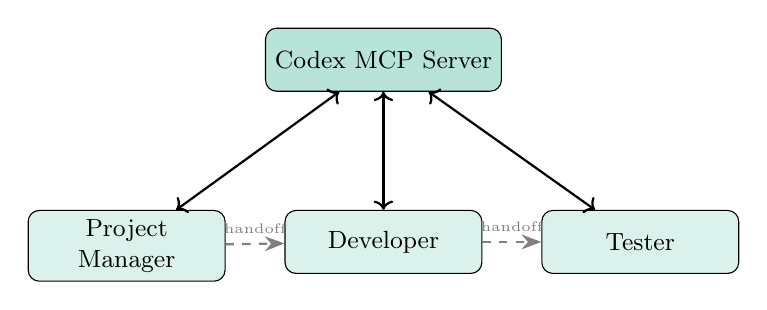
\begin{tikzpicture}[
    node distance=1.2cm,
    box/.style={rectangle, draw, rounded corners, minimum width=2.5cm, minimum height=0.8cm, align=center, font=\small},
    arrow/.style={-{Stealth[length=2.5mm]}, thick}
]
    % MCP Server
    \node[box, fill=codexgreen!30] (mcp) {Codex MCP Server};

    % Agents
    \node[box, fill=codexgreen!15, below left=1.5cm and 0.5cm of mcp] (pm) {Project\\Manager};
    \node[box, fill=codexgreen!15, below=1.5cm of mcp] (dev) {Developer};
    \node[box, fill=codexgreen!15, below right=1.5cm and 0.5cm of mcp] (test) {Tester};

    % Arrows
    \draw[arrow, <->] (mcp) -- (pm);
    \draw[arrow, <->] (mcp) -- (dev);
    \draw[arrow, <->] (mcp) -- (test);

    % Handoffs
    \draw[arrow, dashed, gray] (pm) -- node[above, font=\tiny] {handoff} (dev);
    \draw[arrow, dashed, gray] (dev) -- node[above, font=\tiny] {handoff} (test);
\end{tikzpicture}
\caption{CG MCP-Based Architecture}
\end{figure}

\subsection{Agent Configuration}

Codex agents are configured via TOML files at \texttt{\textasciitilde/.codex/agents.toml}:

\begin{lstlisting}[caption=Codex Agent Configuration (agents.toml)]
[agents.code-reviewer]
name = "Code Reviewer"
system_prompt = """
You are an expert code reviewer focusing on:
- Security vulnerabilities
- Performance issues
- Code quality and maintainability
"""
model = "gpt-5"

[agents.security-auditor]
name = "Security Auditor"
system_prompt = "You are a security specialist..."
\end{lstlisting}

\subsection{Multi-Agent Orchestration}

\begin{codexbox}[Codex Orchestration Features]
\begin{itemize}
    \item \textbf{Hierarchical Coordination}: Project Manager gates handoffs
    \item \textbf{Parallel Execution}: Independent agents run concurrently
    \item \textbf{File-Based Checkpoints}: Deliverables gate progression
    \item \textbf{Bidirectional Handoffs}: Return to PM for validation
\end{itemize}
\end{codexbox}

\subsubsection{Agents SDK Integration}

\begin{lstlisting}[language=python, caption=Codex + Agents SDK]
from agents import Agent, Runner
from agents.mcp import MCPServerStdio

async with MCPServerStdio(
    name="Codex CLI",
    params={"command": "npx", "args": ["-y", "codex", "mcp"]},
) as codex_mcp:

    developer = Agent(
        name="Developer",
        instructions="Build features based on specs...",
        mcp_servers=[codex_mcp],
        model="gpt-5"
    )

    reviewer = Agent(
        name="Reviewer",
        instructions="Review code quality...",
        mcp_servers=[codex_mcp],
        handoffs=[developer]
    )

    result = await Runner.run(reviewer, task)
\end{lstlisting}

\subsection{Sandbox and Permissions}

\begin{table}[h]
\centering
\begin{tabular}{ll}
\toprule
\textbf{Setting} & \textbf{Description} \\
\midrule
\texttt{approval-policy: never} & Autonomous execution \\
\texttt{approval-policy: always} & Require user approval \\
\texttt{sandbox: workspace-write} & Write within workspace only \\
\texttt{sandbox: none} & Full system access \\
\bottomrule
\end{tabular}
\caption{Codex Sandbox Configuration}
\end{table}

%==============================================================================
\section{CCG + CG Coordination Architecture}
%==============================================================================

\subsection{Hybrid Orchestration Model}

The Miyabi platform coordinates CCG and CG through a unified orchestration layer:

\begin{figure}[h]
\centering
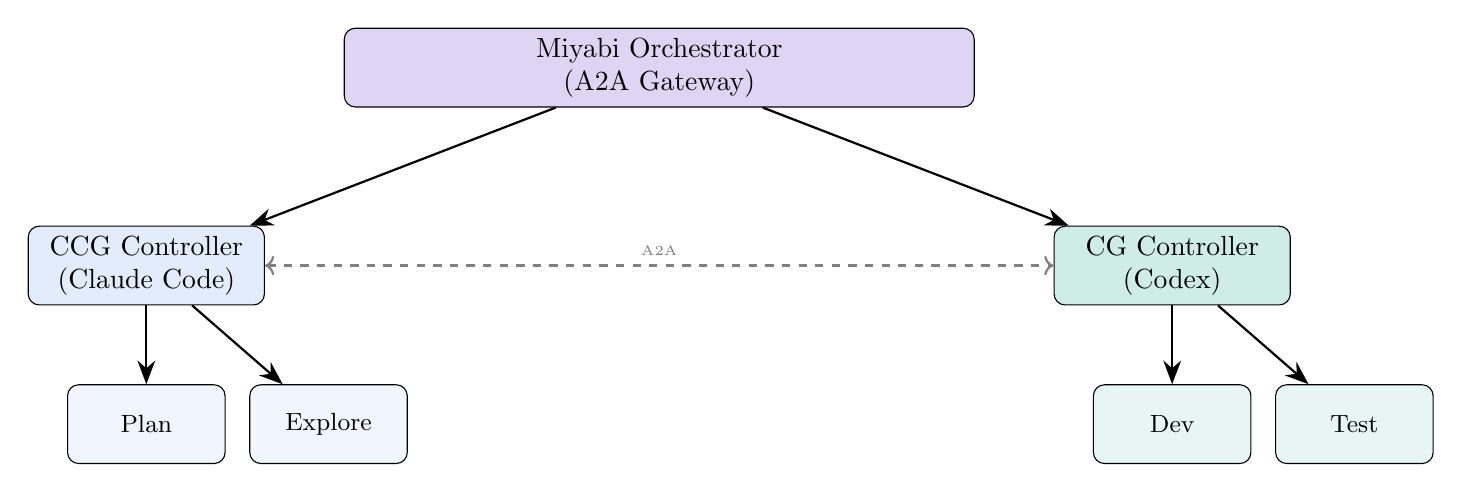
\begin{tikzpicture}[
    node distance=1cm,
    box/.style={rectangle, draw, rounded corners, minimum width=3cm, minimum height=1cm, align=center},
    arrow/.style={-{Stealth[length=3mm]}, thick}
]
    % Miyabi Orchestrator
    \node[box, fill=miyabipurple!30, minimum width=8cm] (orch) {Miyabi Orchestrator\\(A2A Gateway)};

    % CCG Side
    \node[box, fill=claudeblue!20, below left=1.5cm and 1cm of orch] (ccg) {CCG Controller\\(Claude Code)};
    \node[box, fill=claudeblue!10, below=1cm of ccg, minimum width=2cm, font=\small] (ccg1) {Plan};
    \node[box, fill=claudeblue!10, right=0.3cm of ccg1, minimum width=2cm, font=\small] (ccg2) {Explore};

    % CG Side
    \node[box, fill=codexgreen!20, below right=1.5cm and 1cm of orch] (cg) {CG Controller\\(Codex)};
    \node[box, fill=codexgreen!10, below=1cm of cg, minimum width=2cm, font=\small] (cg1) {Dev};
    \node[box, fill=codexgreen!10, right=0.3cm of cg1, minimum width=2cm, font=\small] (cg2) {Test};

    % Arrows
    \draw[arrow] (orch) -- (ccg);
    \draw[arrow] (orch) -- (cg);
    \draw[arrow] (ccg) -- (ccg1);
    \draw[arrow] (ccg) -- (ccg2);
    \draw[arrow] (cg) -- (cg1);
    \draw[arrow] (cg) -- (cg2);

    % Cross communication
    \draw[arrow, <->, dashed, gray] (ccg) -- node[above, font=\tiny] {A2A} (cg);
\end{tikzpicture}
\caption{Miyabi Hybrid CCG/CG Architecture}
\end{figure}

\subsection{Role Definitions}

\begin{table}[h]
\centering
\begin{tabular}{llll}
\toprule
\textbf{Role} & \textbf{System} & \textbf{Responsibility} & \textbf{Strengths} \\
\midrule
Coordinator & CCG & Task decomposition, DAG & Long context, reasoning \\
Planner & CCG & Architecture design & Planning mode \\
Explorer & CCG & Codebase analysis & Fast Haiku search \\
Developer & CG & Code generation & GPT-5 creativity \\
Tester & CG & Test creation & Structured output \\
Reviewer & CCG & Quality assurance & Opus deep analysis \\
\bottomrule
\end{tabular}
\caption{Hybrid Agent Role Assignment}
\end{table}

\subsection{Coordination Patterns}

\subsubsection{Pattern 1: Sequential Handoff}

\begin{lstlisting}[caption=Sequential CCG to CG Handoff]
# Phase 1: CCG Planning
plan = await ccg_planner.query("Analyze and design feature X")

# Phase 2: CG Implementation
impl = await cg_developer.query(f"Implement: {plan}")

# Phase 3: CCG Review
review = await ccg_reviewer.query(f"Review: {impl}")
\end{lstlisting}

\subsubsection{Pattern 2: Parallel Execution}

\begin{lstlisting}[caption=Parallel CCG and CG Execution]
# Run CCG and CG agents in parallel
results = await asyncio.gather(
    ccg_explore.query("Search for auth patterns"),
    cg_developer.query("Generate auth boilerplate"),
    ccg_security.query("Review security requirements")
)

# Synthesize results
synthesis = await ccg_coordinator.query(
    f"Synthesize findings: {results}"
)
\end{lstlisting}

\subsubsection{Pattern 3: Competitive Validation}

\begin{lstlisting}[caption=Cross-System Validation]
# Generate with one system
ccg_impl = await ccg_developer.query("Implement feature")

# Validate with the other
cg_review = await cg_reviewer.query(f"Review: {ccg_impl}")

# Or vice versa
cg_impl = await cg_developer.query("Implement feature")
ccg_review = await ccg_reviewer.query(f"Review: {cg_impl}")
\end{lstlisting}

\subsection{A2A Protocol Integration}

Miyabi's A2A protocol enables standardized communication:

\begin{lstlisting}[caption=A2A Tool Naming Convention]
# CCG agents
a2a.claude_code_planning_agent.analyze_architecture
a2a.claude_code_review_agent.review_code

# CG agents
a2a.codex_development_agent.generate_code
a2a.codex_testing_agent.create_tests

# Cross-system routing via A2A Gateway
a2a_gateway.route(
    source="ccg.planner",
    target="cg.developer",
    payload=plan_document
)
\end{lstlisting}

%==============================================================================
\section{Implementation Guidelines}
%==============================================================================

\subsection{Miyabi Integration Steps}

\begin{enumerate}
    \item \textbf{Configure CCG Agents}
    \begin{itemize}
        \item Create \texttt{.claude/agents/} directory
        \item Define agent specs with YAML frontmatter
        \item Set up Claude Agent SDK hooks
    \end{itemize}

    \item \textbf{Configure CG Agents}
    \begin{itemize}
        \item Create \texttt{\textasciitilde/.codex/agents.toml}
        \item Define agent system prompts
        \item Configure MCP server integration
    \end{itemize}

    \item \textbf{Implement A2A Gateway}
    \begin{itemize}
        \item Register both CCG and CG agents
        \item Define routing rules
        \item Implement message transformation
    \end{itemize}

    \item \textbf{Create Orchestration Workflows}
    \begin{itemize}
        \item Define task decomposition rules
        \item Implement parallel execution handlers
        \item Set up result aggregation
    \end{itemize}
\end{enumerate}

\subsection{Configuration Files}

\subsubsection{CCG Configuration (.claude/agents/miyabi-coordinator.md)}

\begin{lstlisting}
---
name: miyabi-coordinator
description: "Miyabi task coordinator with CCG/CG routing"
model: opus
tools:
  - Read
  - Glob
  - Grep
  - Task
  - Bash
permissionMode: default
---

You are the Miyabi Coordinator responsible for:
1. Decomposing tasks into subtasks
2. Routing tasks to CCG or CG agents
3. Aggregating results
4. Managing cross-system handoffs
\end{lstlisting}

\subsubsection{CG Configuration (\textasciitilde/.codex/agents.toml)}

\begin{lstlisting}[language=python]
[agents.miyabi-developer]
name = "Miyabi Developer"
system_prompt = """
You are a Miyabi development agent specializing in:
- Feature implementation
- Code generation
- Test creation

Always output to designated folders and create checkpoints.
"""
model = "gpt-5"
\end{lstlisting}

\subsection{MCP Server Setup}

\begin{lstlisting}[language=json, caption=.mcp.json Configuration]
{
  "servers": {
    "miyabi-ccg": {
      "command": "claude-code",
      "args": ["mcp"],
      "protocol": "stdio"
    },
    "miyabi-cg": {
      "command": "npx",
      "args": ["-y", "codex", "mcp"],
      "protocol": "stdio"
    }
  }
}
\end{lstlisting}

%==============================================================================
\section{Best Practices}
%==============================================================================

\subsection{Orchestration Guidelines}

\begin{warningbox}[Critical Rules]
\begin{enumerate}
    \item \textbf{Pure Orchestrator}: The coordinator must NOT do actual work
    \item \textbf{No Nested Subagents}: CCG subagents cannot spawn subagents
    \item \textbf{Respect Parallelism Limits}: Max 10 CCG tasks, variable for CG
    \item \textbf{Context Isolation}: Do not share full history between systems
\end{enumerate}
\end{warningbox}

\subsection{Task Routing Heuristics}

\begin{table}[h]
\centering
\begin{tabular}{lll}
\toprule
\textbf{Task Type} & \textbf{Recommended System} & \textbf{Reason} \\
\midrule
Long-form analysis & CCG (Opus) & 200k context window \\
Fast exploration & CCG (Haiku) & Speed-optimized \\
Code generation & CG (GPT-5) & Creative output \\
Structured output & CG & JSON mode support \\
Security review & CCG (Opus) & Deep reasoning \\
Test generation & CG & Template-based \\
Documentation & CCG & Long-form writing \\
\bottomrule
\end{tabular}
\caption{Task Routing Recommendations}
\end{table}

\subsection{Error Handling}

\begin{lstlisting}[language=python, caption=Robust Error Handling]
async def execute_hybrid_task(task):
    try:
        # Try CCG first
        result = await ccg_agent.query(task, timeout=300)
    except CCGTimeoutError:
        # Fallback to CG
        result = await cg_agent.query(task)
    except Exception as e:
        # Log and escalate
        await a2a_gateway.escalate(task, error=e)
        raise

    return result
\end{lstlisting}

\subsection{Monitoring and Observability}

\begin{itemize}
    \item Enable logging on both CCG and CG agents
    \item Use hooks to track tool usage
    \item Implement cost tracking per agent system
    \item Monitor context window utilization
    \item Track cross-system latency
\end{itemize}

%==============================================================================
\section{Limitations and Constraints}
%==============================================================================

\subsection{CCG Limitations}

\begin{itemize}
    \item No subagent nesting (prevents infinite complexity)
    \item Maximum 10 concurrent tasks
    \item No direct peer communication between subagents
    \item Batch queue waits for completion before pulling next
\end{itemize}

\subsection{CG Limitations}

\begin{itemize}
    \item Requires MCP server for agent integration
    \item Session persistence depends on MCP connection
    \item Sandbox restrictions may limit file access
    \item Model availability varies by plan
\end{itemize}

\subsection{Cross-System Constraints}

\begin{itemize}
    \item No native inter-system communication
    \item Context must be explicitly passed between systems
    \item Different authentication mechanisms
    \item Varying response formats require normalization
\end{itemize}

%==============================================================================
\section{Conclusion}
%==============================================================================

The CCG + CG coordination architecture enables Miyabi to leverage the strengths of both Claude Code and OpenAI Codex:

\begin{itemize}
    \item \textbf{CCG} excels at planning, analysis, and deep reasoning with large context windows
    \item \textbf{CG} excels at code generation and structured workflows via MCP
    \item \textbf{Miyabi's A2A Gateway} provides the bridge for seamless coordination
\end{itemize}

By following the patterns and guidelines in this document, development teams can build sophisticated multi-agent workflows that combine the best of both AI systems.

%==============================================================================
\section*{References}
%==============================================================================

\begin{enumerate}
    \item Claude Code Documentation: \url{https://docs.anthropic.com/claude-code}
    \item Claude Agent SDK: \url{https://github.com/anthropics/claude-agent-sdk-python}
    \item OpenAI Codex: \url{https://github.com/openai/codex}
    \item Codex Agents SDK Guide: \url{https://developers.openai.com/codex/guides/agents-sdk}
    \item Miyabi A2A Protocol: Internal Documentation
\end{enumerate}

\end{document}
